%-----------------------------------------------------------------
%	ROTACIÓ DE LA VIA LÀCTIA
%	!TEX root = ./../main.tex
%-----------------------------------------------------------------
\section{Rotació de la Via Làctia}
%-----------------------------------------------------------------
\subsection{El disc i l'halo de la Via Làctia}
El disc de la Galàxia ha estat objecte d'un estudi més detallat que l'halo.

Al disc les estrelles i els núvols de gas interestel·lar es desplacen en orbites aproximadament circulars en torn al centre de la Galàxia (figura \ref{fig:orbit-star}). La rotació no és uniforme (de sòlid rígid) sinó que les estrelles més properes al centre inverteixen menys temps que les més llunyanes en completar una volta (rotació diferencial $\Omega = \Omega(r)$, figura \ref{fig:star-pattern}).

\begin{figure}[h]
	\centering
	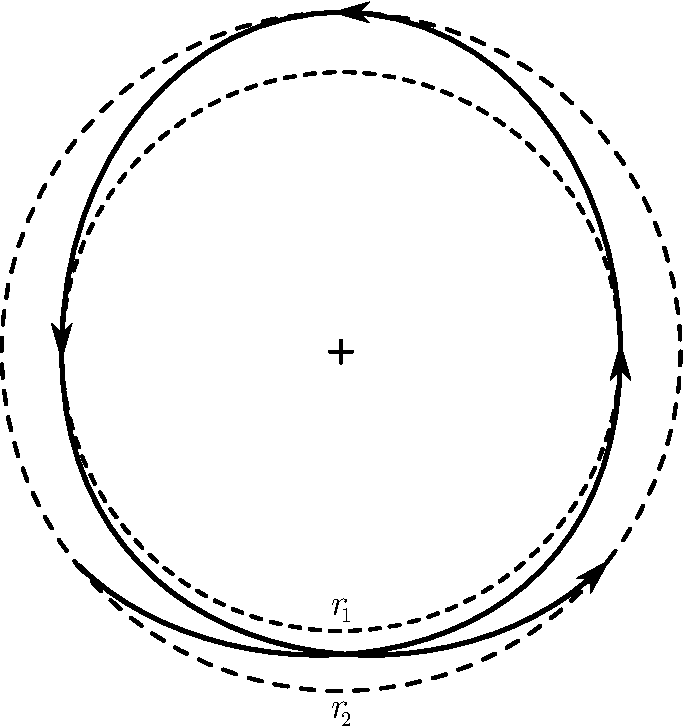
\includegraphics[width=0.55\textwidth]{./images/7-orbit-star}
	\caption{Òrbita d'una estrella projectada sobre el pla del disc. El radi de entre $r_{1}$ i $r_{2}$. El temps invertit en tornar a la distància $r_{2}$ després d'haver partit d'allà és, en general, menor que el temps en completar una volta. L'òrbita no és tancada}
	\label{fig:orbit-star}
\end{figure}

\begin{figure}[h]
	\centering
	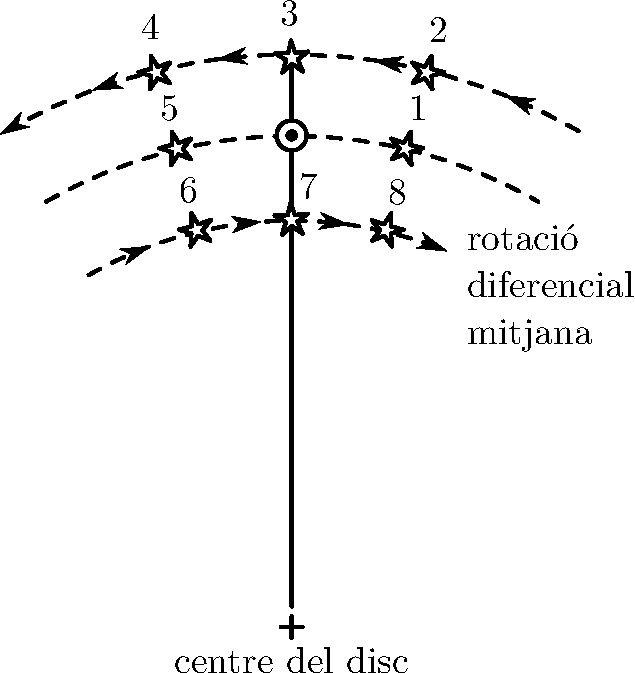
\includegraphics[width=0.45\textwidth]{./images/7-star-pattern}
	\caption{Patró de moviment típic de rotació d'estrelles situades a uns pocs milers d'any llum del Sol ($\odot$)}
	\label{fig:star-pattern}
\end{figure}

La velocitat del Sol en la seva òrbita és $\approx \SI{220}{\km \per\s}$ i el seu període $\approx \SI{200}{\mega\year}$ (si l'edat del Sol és $\approx \SI{5e9}{\year}$, haurà completat la seva òrbita unes 25 vegades).

Les estrelles i núvols de gas propers al Sol viatgen aproximadament a la velocitat d'aquest, de manera que estan gairebé en repòs respecte al Sol. En astronomia es defineix el Sistema de referència estàndard local (\textit{Local Standard of Rest}, LSR) com aquell que segueix el moviment mitjà del material del disc en la velocitat del Sol.

No obstant això, hi ha estrelles a les proximitats del Sol que posseeixen una velocitat notable respecte al LSR. Es dóna el fet curiós que aquestes tenen la seva velocitat cap a una direcció i no cap a l'oposada (figura \ref{fig:asimetria-estrelles}).
\begin{figure}[H]
	\centering
	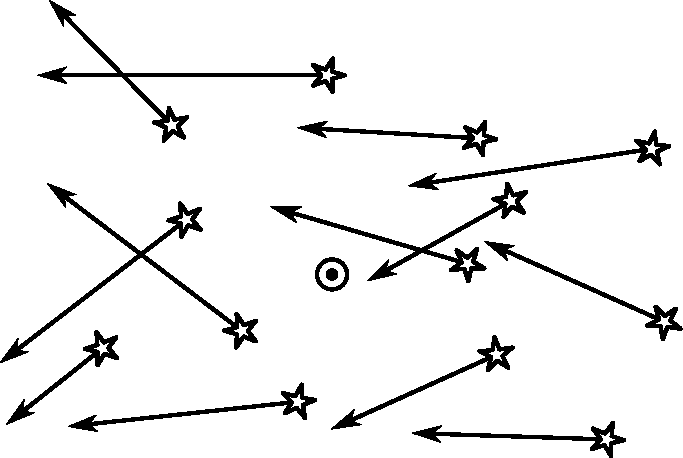
\includegraphics[width=0.5\textwidth]{./images/7-asimetria-estrelles}
	\caption{Asimetria de les estrelles d'\textit{alta velocitat}. Les estrelles que es desplacen a velocitats superiors a $\SI{65}{\km \per\s}$ respecte del sistema estàndard local semblen desplaçar-se exclusivament de dreta a esquerra. No es coneixen estrelles d'alta velocitat que es desplacen al sentit oposat}
	\label{fig:asimetria-estrelles}
\end{figure}

L'explicació d'aquest fenomen és deguda a Lindblad (1895--1965): les estrelles d'alta velocitat posseeixen en realitat baixa velocitat rotacional i gran velocitat no rotacional. El Sol (i altres estrelles) giren ràpidament deixant-les al darrere per la qual cosa les d'\textit{alta velocitat} semblen fluir en sentit oposat. Nosaltres tenim a considerar al Sol en repòs, però si l'observem des del centre de la Galàxia, comprovaríem que les estrelles d'\textit{alta velocitat} posseeixen en realitat un moviment més lent que el Sol.

La figura \ref{fig:star-pattern} mostra que, en mitjana, les estrelles situades entre el Sol i el centre del disc inverteixen menys temps que aquest en completar una òrbita en torn al centre del disc, mentre que les situades més lluny al centre que el Sol inverteixen més temps. Aquesta rotació diferencial recolza la tesi que el Sol no és al centre de la Galàxia.

Mesures observacionals permeten determinar el cisallament (\textit{shear}) de la rotació diferencial en l'entorn del Sol i la \textit{vorticitat}. Aquestes magnituds venen donades a través de les constants $A$ i $B$ de Oort definides per
\begin{align}
	A = - \frac{r}{2} \dv{\Omega}{r} \qc B = -\frac{1}{2r} \dv{\qty(r^{2}\Omega)}{r},
\end{align}
de manera que
\begin{align}
	\Omega = A - B
\end{align}

Observacionalment es troba que
\begin{align*}
	A = \SI{0.005}{\km \per\s \per\lightyear} \qc \sqrt{1 - A/B} = 1.6
\end{align*}
La constant $A$ mesura el cisallament i s'obté de mesures de les velocitats radials al veïnatge solar. A la vegada, mesures de moviments propis mitjans ens donen la constant $B$ (vorticitat). Com la figura \ref{fig:vel-erratic} indica, en les proximitats del Sol, les estrelles tenen velocitats erràtiques predominantment orientades cap al centre de la Galàxia. Conegudes $A$ i $B$ es determina $\Omega$, i el període $2\pi/\Omega$ (aproximadament 220 milions d'anys per a estrelles properes al Sol). Això, juntament amb la distància del Sol al centre del disc ($\approx \SI{25}{\giga\lightyear}$), ens permet determinar la velocitat orbital del Sol en aproximadament $\SI{220}{\km\per\s}$.

\begin{figure}[h]
	\centering
	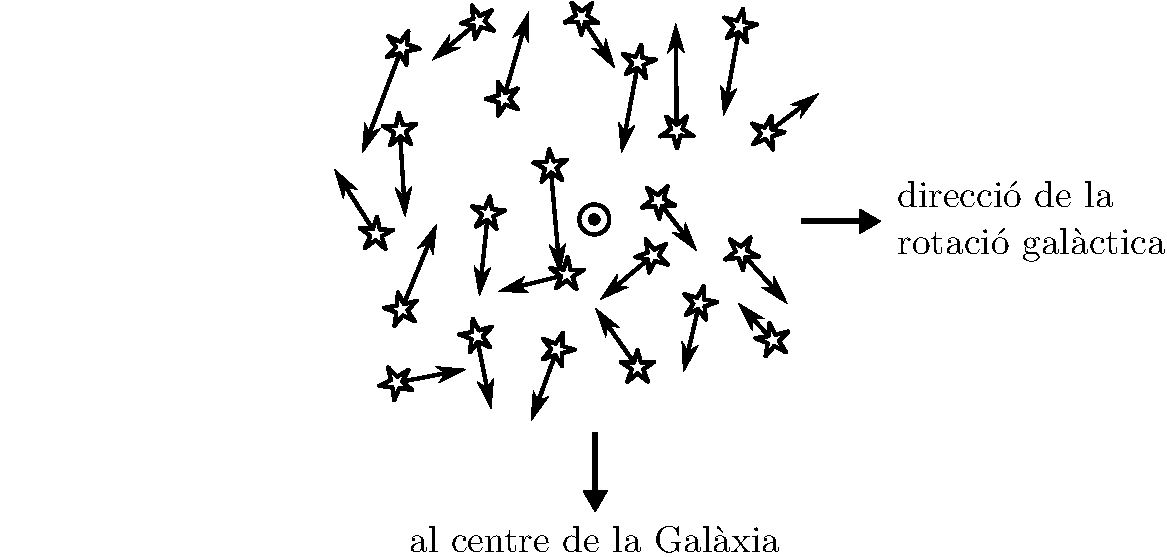
\includegraphics[width=0.8\textwidth]{./images/7-vel-erratic}
	\caption{Les velocitats erràtiques de les estrelles al veïnatge del Sol tendeixen a ser majors cap al centre de la Galàxia que en la direcció de rotació. Aquesta asimetria en la dispersió de velocitats també mostra que la Galàxia no gira com sòlid rígid}
	\label{fig:vel-erratic}
\end{figure}

Tanmateix, es pot estimar la massa de la Galàxia interior a l'òrbita solar com $M(r) = v^{2} r / G \approx \SI{e11}{\Msun} > M_{lluminosa}$.

Malgrat l'enorme nombre d'estrelles a la Galàxia, una col·lisió és altament improbable (excepte, és clar, en sistemes lligats: estrelles binàries, cúmuls d'estrelles; o al centre de la Via Làctia).

\subsubsection*{Coordenades galàctiques}
Per descriure el moviment de les estrelles al disc convé introduir dos sistemes de coordenades diferents (figura \ref{fig:coordenades-galactiques}):
\begin{itemize}
	\item Un sistema de coordenades cilíndriques $(r, \theta, z)$ amb origen al centre del disc (útil per a la descripció teòrica).
	\item Un sistema $(R,l,b)$ centrat al Sol (útil per a la descripció observacional), on $R$, és la distància al Sol, $l$ la longitud, i $b$ la latitud.
\end{itemize}

\begin{figure}[h]
	\centering
	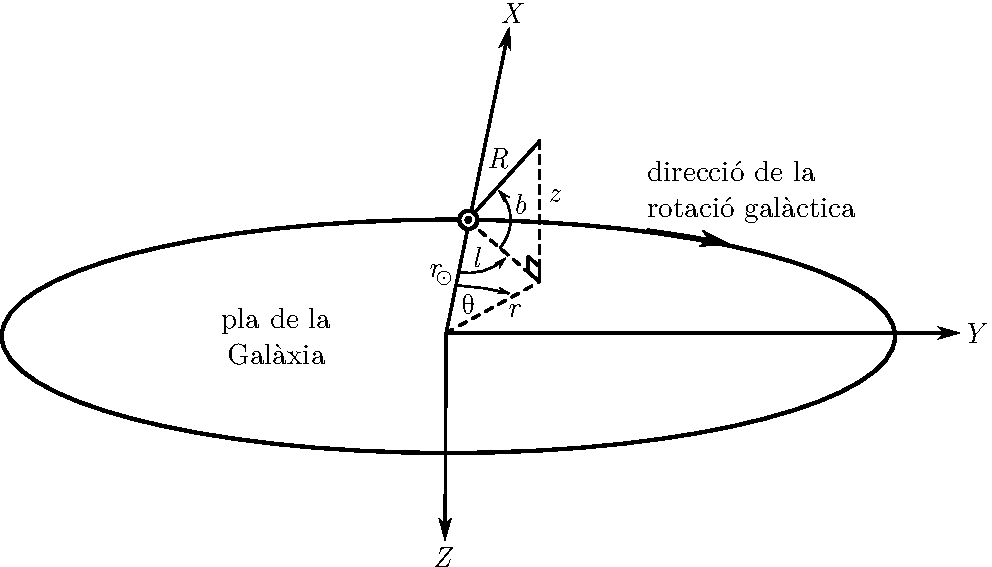
\includegraphics[width=0.9\textwidth]{./images/7-coordenades-galactiques}
	\caption{Coordenades galàctiques. Els astrònoms acostumen a presentar les seves observacions al pla galàctic com si el contempléssim de dalt cap a baix. Llavors, als dibuixos observacionals el sentit de rotació de la Galàxia en torn a l'eix $Z$ és el sentit horari}
	\label{fig:coordenades-galactiques}
\end{figure}

\subsubsection*{Òrbites estel·lars al disc}
A ordre zero, el camp gravitatori al disc resulta estacionari (independent del temps) i amb simetria axial. Per tant, dins d'aquesta aproximació, l'energia per unitat de massa i el moment angular per unitat de massa són constants del moviment.
\begin{align*}
	E = \frac{1}{2} \qty(v_{r}^{2} + v_{\theta}^{2} + v_{z}^{2}) + V(r,z) \approx cte \qc J = r v_{\theta} \approx cte
\end{align*}

Tenint això en compte, les òrbites al disc no són exactament circulars: superimposat al moviment circular es dóna un altre segons l'el·lpse centrada al cercle i en sentit retrògrad; és a dir, es tracta d'un \textit{epicicle} (figura \ref{fig:galaxy-epicycle}) tal que les freqüències angulars d'ambdós moviments ($\kappa$ i $\Omega$) difereixen en general. Per una altra part, la freqüència del moviment alllarg de l'eix $z$ és major que $\kappa$ i $\Omega$.
\begin{figure}[h]
	\centering
	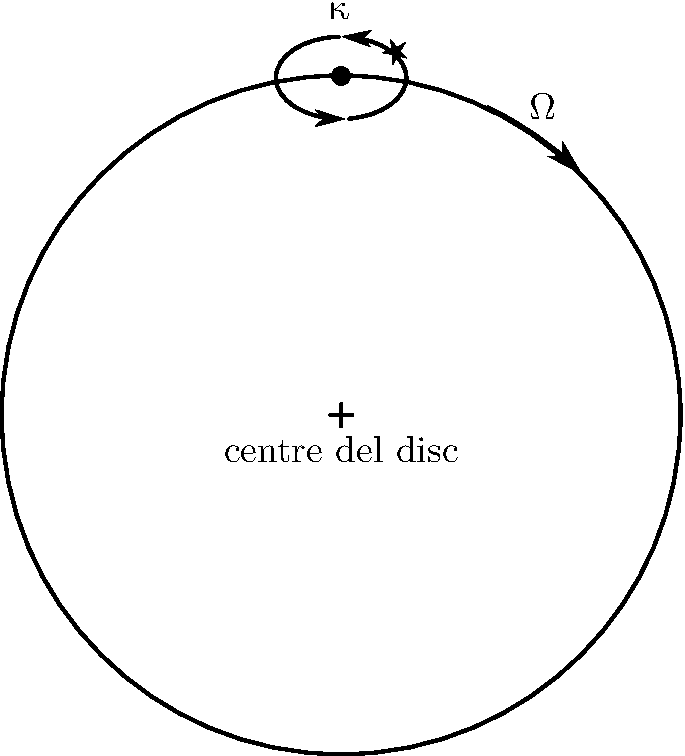
\includegraphics[width=0.5\textwidth]{./images/7-galaxy-epicycle}
	\caption{Epicicle. Si l'òrbita és lleugerament no circular, aquesta pot entendre's com formada per la superposició d'un moviment circular de velocitat angular constant $\Omega$, i un moviment retrògrad, el·líptic de freqüència $\kappa$ amb centre al cercle}
	\label{fig:galaxy-epicycle}
\end{figure}

Per conèixer l'estructura de la Galàxia a gran escala (i d'això dedir la seva distribució de massa) hem de determinar la posició i velocitat de rotació d'objectes molt llunyans al Sol. En aquesta tasca ens servim de la longitud d'ona de $\SI{21}{\cm}$ de l'hidrogen atòmic.

Suposem un radiotelescopi localitzat al Sol i apuntant en la direcció de la longitud galàctica $l$ amb $b = 0$. A la figura \ref{fig:patro-rotacio} s'adverteix que el núvol de gas 2 és d'especial interès, ja que només hi ha un punt tangent (o punt subcentral).

A causa de la rotació diferencial, el núvol 2 (més proper que els altres de la figura \ref{fig:patro-rotacio} al centre de la Galàxia) es mou amb major velocitat que els altres núvols respecte a nosaltres. Els núvols 1 i 3 s'allunyen més lentament, el núvol 4 apareix amb velocitat zero ja que es troba a igual distància que el Sol al centre de la Galàxia, i el núvol 5 (extern a l'òrbita del Sol) s'aproxima a nosaltres (posseeix velocitat radial negativa). El cas del núvol 2 és molt especial ja que
\begin{align*}
	r = r_{\odot} \sin l
\end{align*}
on $r_{\odot}$ és la distància del Sol al centre de la Galàxia ($\approx \SI{8.5}{\kilo\parsec}$).
\begin{figure}[H]
	\centering
	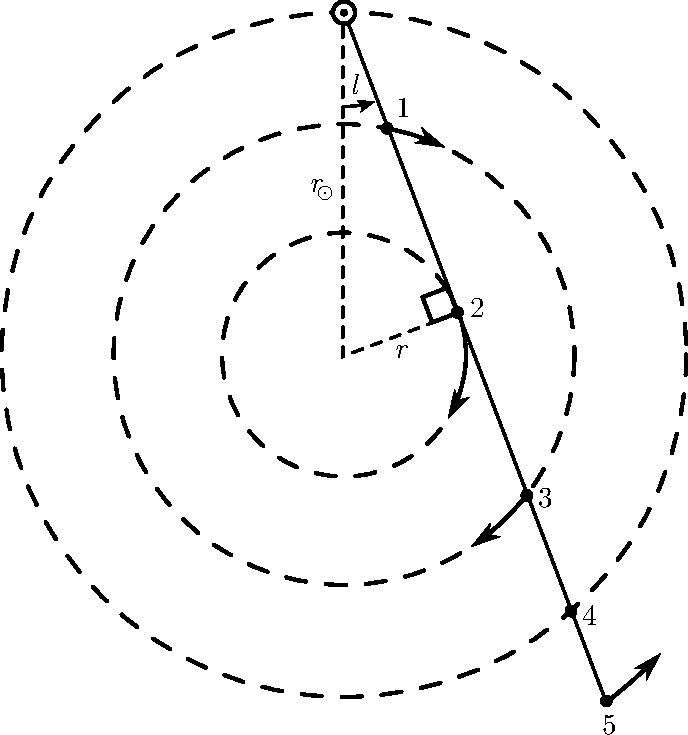
\includegraphics[width=0.6\textwidth]{./images/7-patro-rotacio}
	\caption{Patró de rotació diferencial a gran escala per a un observador al sistema local de referència. Cal notar que els núvols 1 i 3 posseeixen igual velocitat al llarg de la visual (velocitat radial), i el núvol 2 té la velocitat radial positiva major; el núvol 4 apareix en repòs, i el 5 posseeix una velocitat negativa}
	\label{fig:patro-rotacio}
\end{figure}

\begin{figure}[H]
	\centering
	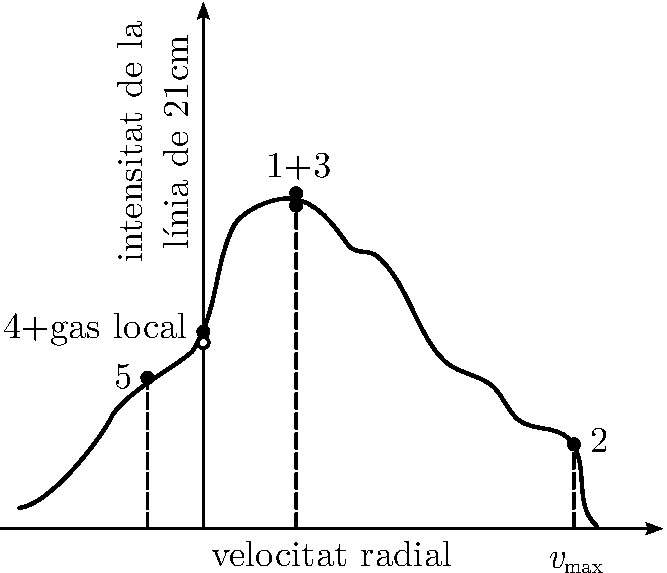
\includegraphics[width=0.47\textwidth]{./images/7-perfil-21cm}
	\caption{Perfil esquemàtic de la intensitat de la línia de $\SI{21}{\cm}$ neutre font a la velocitat radial. La màxima velocitat es dóna per al núvol 2 (al punt de tangència)}
	\label{fig:perfil-21cm}
\end{figure}

Per tant, per trobar les velocitats i posicions d'objectes en òrbites interiors al Sol, l'estratègia és apuntar el radiotelescopi a diferents longituds $l$; així s'obté la velocitat radial $v(r)$ per a diferents distàncies radials (del punt de tangència) al centre de la Via Làctia. El resultat es mostra a la figura \ref{fig:gal-corba-rotacio1}, corba de rotació de la Galàxia.
\begin{figure}[H]
	\centering
	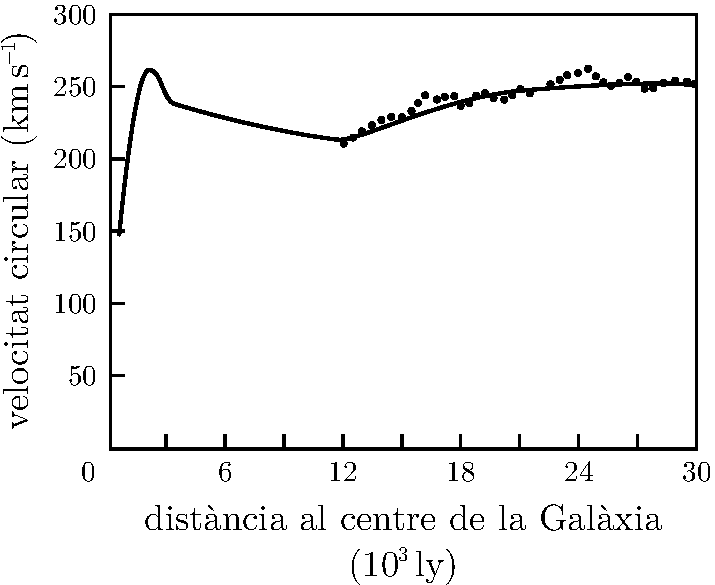
\includegraphics[width=0.51\textwidth]{./images/7-gal-corba-rotacio1}
	\caption{Corba de rotació de la Galàxia obtinguda mitjançant observacions de $\lambda = \SI{21}{\cm}$ de l'àtom d'hidrogen per a núvols de gas interiors al cercle solar}
	\label{fig:gal-corba-rotacio1}
\end{figure}

Com que més enllà del cercle solar no hi ha punts tangents, aquest mètode només serveix per a objectes que es mouen en òrbites interiors a aquest cercle.

La corba de rotació de la Galàxia per a objectes que es mouen en òrbites externes a la solar s'obté mesurant per mitjans òptics la distància a objectes la velocitat radial de les quals es desitja determinar.
\begin{figure}[H]
	\centering
	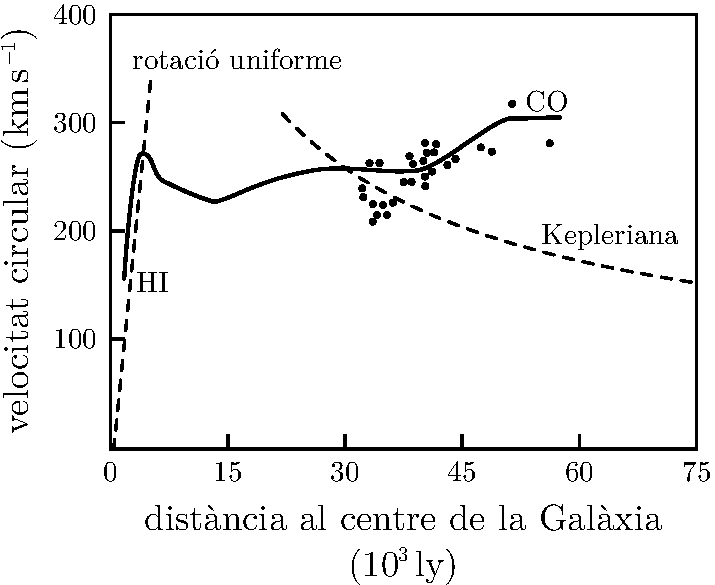
\includegraphics[width=0.51\textwidth]{./images/7-gal-corba-rotacio2}
	\caption{Corba de rotació de la Galàxia estesa més enllà del cercle solar per mitjans fotomètrics d'estrelles OB i emissió de \ch{CO} de núvols moleculars gegants}
	\label{fig:gal-corba-rotacio2}
\end{figure}

Se sol recórrer a complexes H II (hidrogen ionitzat) gegants als límits del disc, ja que experimenten poc enfosquiment degut a la pols interestel·lar i les seves distàncies es poden trobar fotomètricament (tot i que no amb gran exactitud) estudiant les propietats òptiques de les estrelles que exciten aquests núvols. Núvols moleculars gegants solen acompanyar als complexes H II, i les velocitats radials d'aquests núvols moleculars poden trobar-se a partir de la seva emissió de \ch{CO} (monòxid de carboni). Aquest mètode permet estendre la corba de rotació de la Galàxia fins a gairebé $\SI{2}{r_{\odot}}$. La corba completa es mostra a la figura \ref{fig:gal-corba-rotacio2}. És obvi que la rotació de la Galàxia és diferencial.

\subsubsection*{Espessor de la capa de gas}
El mètode del punt tangent (al qual li correspon la màxima velocitat al llarg de la visual, per a una longitud $l$ fixa) se suposa vàlid fins i tot encara si la coordenada angular $b$ és lleugerament diferent de zero. Mitjançant l'estudi del descens en intensitat de la línia $\SI{21}{\cm}$ d'hidrogen atòmic conforme el radiotelescopi escombra diferents valors de $b$ (latitud galàctica) tot mantenint $l$ (longitud), els astrònoms mesuren l'amplada efectiva dels punts de tangència.

Es troba que la capa d'hidrogen presenta una amplada pràcticament constant d'uns $\SI{700}{\lightyear}$ ($\approx \SI{214}{\parsec}$) per a tots els radis interiors a l'òrbita solar.

Mesures anàlogues s'han portat a terme per a mesuraments de \ch{CO} per les distribucions de gas molecular, trobant que aquest posseeix una amplada de $\SI{300}{\lightyear}$ ($\approx \SI{92}{\parsec}$). Com que el diàmetre del cercle solar és d'aproximadament $\SI{5 e4}{\lightyear}$, veiem que les capes de gas i pols a la Via Làctia són proporcionalment tan primes com un naip.

Es coneix que la capa d'hidrogen atòmic s'estén molt més enllà de l'òrbita solar, mostrant, a més a més, una duplicitat en la seva perifèria (figura \ref{fig:disc-perfil}). Aquest efecte, també observat en altres galàxies, podria atribuir-se al fet que els núvols de Magalhães hagin passat recentment molt a prop de la Galàxia, produint efectes de marea.
\begin{figure}[h]
	\centering
	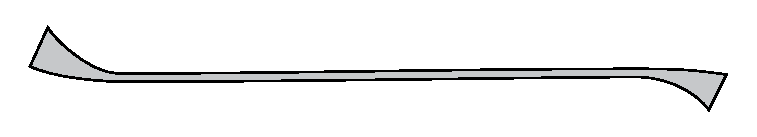
\includegraphics[width=0.65\textwidth]{./images/7-disc-perfil}
	\caption{Vista de perfil (esquemàtica) del disc gasós de la Galàxia mostrant el seu eixamplament més enllà de l'òrbita solar i la seva duplicitat en la perifèria}
	\label{fig:disc-perfil}
\end{figure}

\subsubsection*{Estructura esquemàtica de la Via Làctia}
La figura \ref{fig:galaxy-scheme} mostra una vista esquemàtica de la Galàxia. La protuberància central posseeix un radi d'uns pocs kiloparsecs. El Sol es troba al disc prim a uns $\SI{8}{\kilo\parsec}$ del nucli, que allotja, sembla ser, un forat negre de massa $\approx \SI{4 e6}{\Msun}$ (que experimenta un augment aproximat de $\SI{7e-10}{\Msun \per\year}$).

\begin{figure}[h]
	\centering
	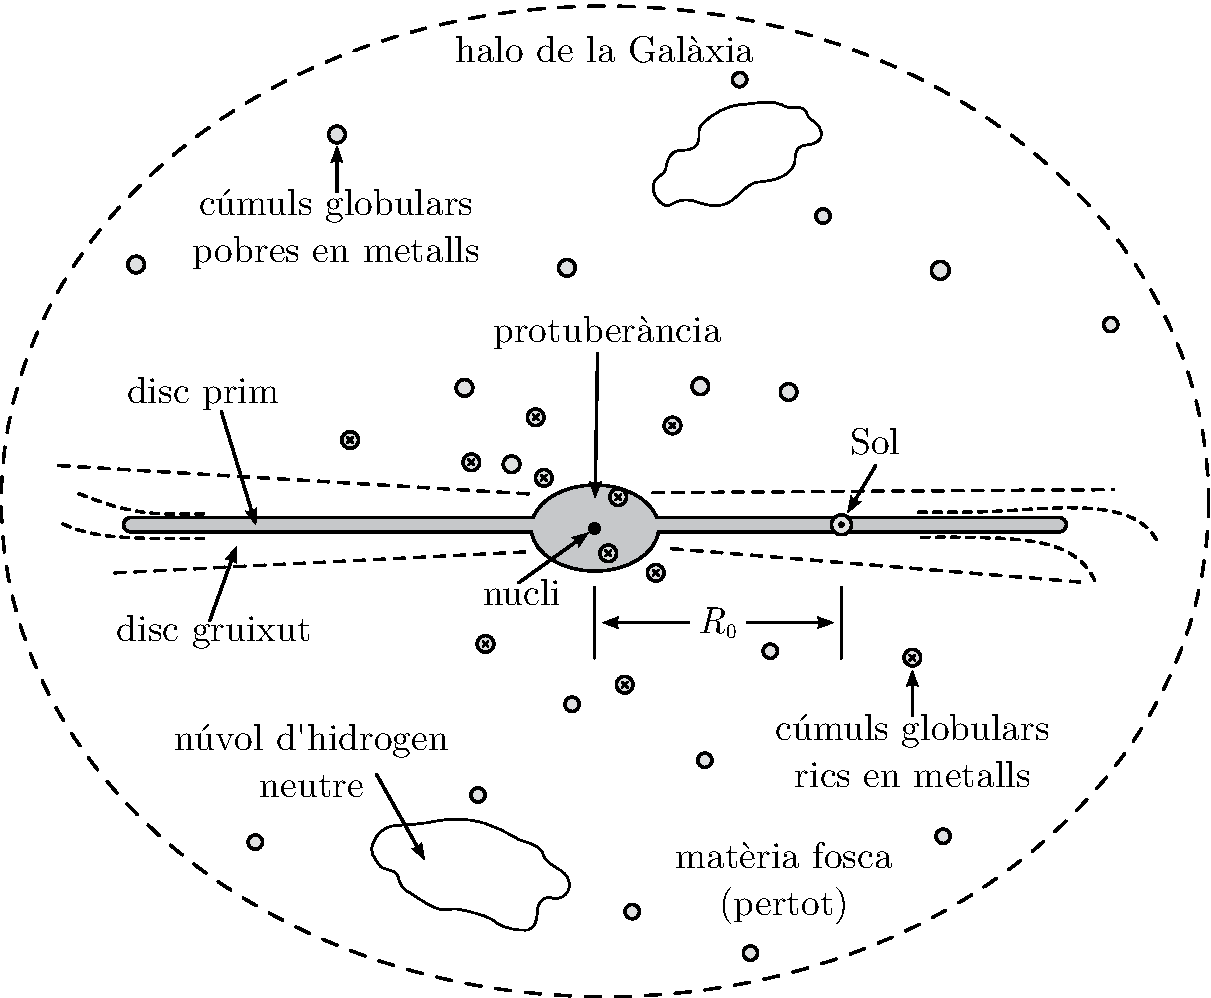
\includegraphics[width=0.8\textwidth]{./images/7-galaxy-scheme}
	\caption{Vista esquemàtica de la Via Làctia}
	\label{fig:galaxy-scheme}
\end{figure}

El \textit{disc prim} conté el 95\% de les estrelles del disc i totes les estrelles massives joves. La seva alçada d'escala (la distància que ens hem de desplaçar perpendicularment al disc perquè la seva densitat caigui en un factor $e$) està entre $\SIrange{300}{400}{\parsec}$. La resta d'estrelles forma el \textit{disc gruixut} amb una alçada d'escala entre $\SIrange{1000}{1500}{\parsec}$. Les estrelles del disc gruixut són més velles que les del disc prim i són més pobres en elements químics pesats. El gas i la pols jeuen en una capa encara més prima que la de les estrelles. Es creu que la matèria fosca se situa per totes parts i també a l'halo de la Galàxia, per aquesta raó és a vegades anomenat l'\textit{halo fosc} (\textit{dark halo}).

%-----------------------------------------------------------------
\subsection{Estructura espiral}
Estudis de la posició i velocitat de núvols de gas hidrogen neutre i núvols moleculars suggereixen que el disc de la Galàxia presenta una estructura espiral de 3 braços semblant a la galàxia NGC 4622 [\href{http://apod.nasa.gov/apod/ap040221.html}{APOD~040221}]. Als braços espirals es dóna una fort concentració de gas i al seu si té lloc la gènesi de noves estrelles. Efectivament, els discs de les galàxies espirals posseeixen un color blau més destacat que ;a resta del disc i les emissions de \ch{H_{$\alpha$}} revelen l'existència de gas calent i ionitzat envoltant estrelles joves massives. Com que estrelles suficientment calents per emetre fotons ultraviolats capaços d'ionitzar àtoms d'hidrogen viuen només 10 milions d'anys, els braços espirals deuen ser llocs on contínuament es formin estrelles. A coordenades galàctiques $(r,l)$ la forma espiral d'una galàxia de $m$ braços es pot representar mitjançant
\begin{align}\label{eq:gal-spirals}
	\cos\qty{m\qty[l + f(r,t)]} = 1
\end{align}
on $f(r,t)$ mesura quant estretament (o no) estan units entre si els braços: si $\abs{\pdv*{f}{r}}$ és gran, els braços estan pegats els uns als altres; si $\abs{\pdv*{f}{r}}$ és petit, llavors estan més oberts. L'angle $i$ entre les tangents al braç espiral i al cercle de radi $r$ que el talla en aquest punt (figura \ref{fig:gal-spiral}) ve donat per
\begin{align}\label{eq:gal-spiral-i}
	\cot i = \abs{r \pdv{l}{r}} = \abs{r \pdv{f}{r}}
\end{align}

\begin{figure}[ht]
	\centering
	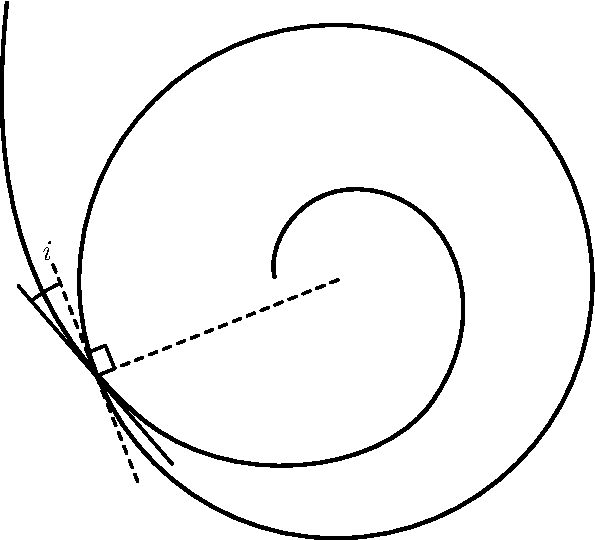
\includegraphics[width=0.5\textwidth]{./images/7-gal-spiral}
	\caption{En un disc que roti en sentit contrari a les agulles del rellotge i en què la velocitat angular $\Omega(r)$ decreixi amb $r$, estrelles inicialment situades al llarg d'un radi es disposarien més tard en una espiral estreta seguint el moviment darrere}
	\label{fig:gal-spiral}
\end{figure}

Es creu que els braços espirals corresponen a ones de densitat; de no ser així, la rotació diferencial de la Galàxia donaria en poc temps que els braços quedessin estrets en un rínxol (cosa que no s'observa). Per veure això amb cert detall suposem que inicialment les estrelles estiguin disposades al llarg d'una línia radial amb $l = l_{0}$ (figura \ref{fig:gal-spiral}). Cada estrella descriu la seva òrbita amb velocitat $v(r)$ (recordem que la velocitat angular és $\Omega(r) = v(r)/r$), de manera que després d'un temps $t$ aquestes estrelles jeuen al llarg de l'espiral
\begin{align*}
	l = l_{0} + \Omega(r) t
\end{align*}
Combinant aquesta expressió amb l'equació \eqref{eq:gal-spirals} se segueix
\begin{align*}
	m \qty[l_{0} + \Omega(r) t + f(r,t)] = 0
\end{align*}
o, equivalentment,
\begin{align}
	f(r,t) = -l_{0} - \Omega(r) t
\end{align}

Com que, en general, $\Omega(r)$ decreix amb $r$, per a $\Omega(r) > 0$ s'infereix que $f(r,t)$ augmenta conforme ens movem al llarg del braç cap a valors de $r$ creixents, així que $l$ ha de disminuir (perquè se segueixi complint l'equació \eqref{eq:gal-spirals}). Tenim, doncs, una \textit{trailing spiral} ja que l'extrem del braç apunta en el sentit oposat al gir; i conforme passa el temps, l'espiral es fa més i més estreta.

Al veïnatge del Sol $v(r)$ ($\approx \SI{220}{\km \per\s}$) és aproximadament constant i $r \approx \SI{8}{\kilo\parsec}$, l'angle $i$ (donat per l'equació \eqref{eq:gal-spiral-i}) s'estrenyeria d'acord amb
\begin{align*}
	\cot i = r \abs{\dv{\Omega(r)}{t}} t \approx \frac{220}{8} \frac{t}{\SI{1}{\giga\year}} \Leftrightarrow i \approx \SI{2}{\degree} \times \qty(\frac{\SI{1}{\giga\year}}{t})
\end{align*}
Després de $\num{e9}$ anys, l'espiral resultaria molt més estreta que les espirals observades a galàxies anàlogues a la Via Làctia. Qualsevol patró inicial patiria un estrenyiment semblant.

El fenomen d'estructura espiral de galàxies és molt complex i probablement siguin varis mecanismes els responsables d'aquest. Un cop el núvol de gas ha produït les primeres estrelles, ones de xoc de les supernoves (corresponents a l'explosió d'estrelles de vida curta) comprimeixen el gas que les envolta. Això pot ocasionar el naixement de més estrelles, així que la producció d'aquestes es propaga a través del gas. A continuació, la rotació diferencial arrossega el núvol a un segment del braç espiral \textit{endarrerit}. Per quan aquest fregament hagi estat fortament estirat, el gas s'haurà esgotat, les estrelles calentes s'hauran apagat i la regió retorna al disc.

Aquest model d'\textit{autopropagació de formació d'estrelles} serà eficaç només si el ritme de naixement d'estrelles pot auto-regular-se de tal manera que no mori mai ni faci cremar tot el disc esgotant el seu gas. Aquest mecanisme pot explicar l'estructura espiral de la galàxia M33, però no probablement la del sistema M100 [\href{http://apod.nasa.gov/apod/ap010203.html}{APOD~010203}], on els braços espirals giren més de $\SI{180}{\degree}$.

Un paràmetre clau en la formació de l'estructura espiral és el paràmetre d'estabilitat de Toomre:
\begin{align}
	Q = \frac{\kappa \sigma_{r}}{3.36 G \Sigma}
\end{align}
on $\kappa$ és la freqüència de l'epicicle (figura \ref{fig:galaxy-epicycle}), $\sigma_{r}$ és la dispersió de velocitats estel·lars al llarg de la visual, i $\Sigma$ és la densitat superficial del disc.

Simulacions mitjançant ordinador mostren que una estructura espiral només apareixerà si $Q \gtrsim 1.2$. Conforme l'estructura espiral es desenvolupa, la mida dels epicicles en les òrbites estel·lars augmenta i amb això $Q$. Així doncs, no s'espera observar una estructura espiral amb $Q < 1$ (figura \ref{fig:gal-simulation}).
\begin{figure}[H]
	\centering
	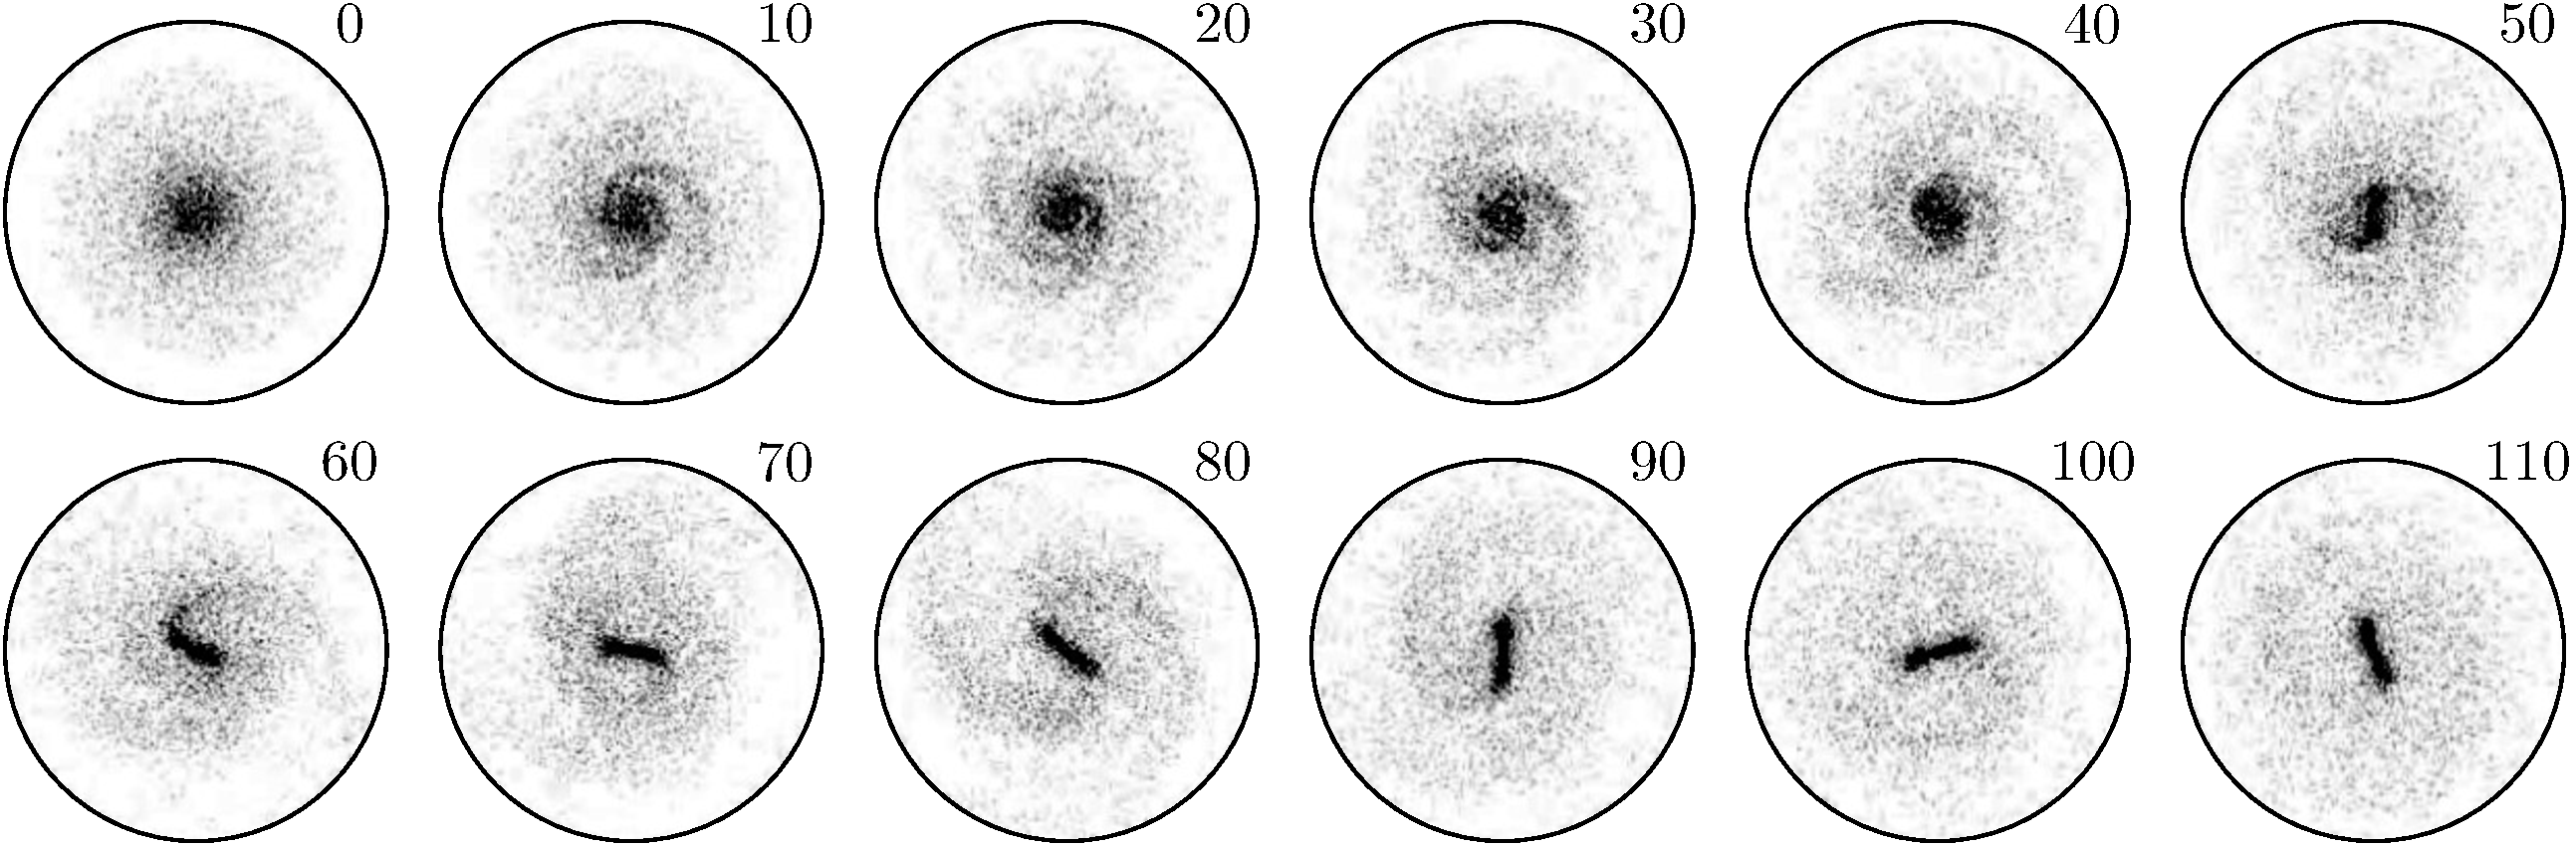
\includegraphics[width=\textwidth]{./images/7-gal-simulation}
	\caption{Simulació per ordinador mostrant com un disc de $\num{50000}$ partícules que s'atreuen mútuament per gravetat desenvolupa primer un patró espiral de dos braços, i després una barra al centre. El bulb galàctic i l'halo fosc són representats per una força cap a dins. La simulació correspon a $\SI{2.65}{\giga\year}$ si el radi del disc és de $\SI{16}{\kilo\parsec}$ i la massa de la galàxia és de $\SI{2 e11}{\Msun}$; el disc comença amb $Q = 1$}
	\label{fig:gal-simulation}
\end{figure}

Al veïnatge solar, i per a estrelles d'edat semblant al Sol ($\approx \SI{5 e9}{\year}$) es té $\sigma_{r} \approx \SI{30}{\km \per\s}$, $\Sigma \approx \SI{50}{\Msun \per\square\parsec}$, $\kappa \approx \SI{36}{\km \per\s \per\kilo\parsec}$, de manera que $Q \approx 1.4$, valor compatible amb l'estructura espiral.
